% This is samplepaper.tex, a sample chapter demonstrating the
% LLNCS macro package for Springer Computer Science proceedings;
% Version 2.20 of 2017/10/04
%

\documentclass[runningheads]{llncs}
%
\usepackage[pdftex]{graphicx}
\usepackage{subfigure}
\usepackage{dirtytalk}
\usepackage{float}
\usepackage[toc,page]{appendix}

\usepackage{graphicx}
% Used for displaying a sample figure. If possible, figure files should
% be included in EPS format.
%
% If you use the hyperref package, please uncomment the following line
% to display URLs in blue roman font according to Springer's eBook style:
% \renewcommand\UrlFont{\color{blue}\rmfamily}

\begin{document}
%
\title{Mr. Caduceus: Predicting Diseases Using Patient Data for Health-Adjusted Taxation }
%
%\titlerunning{Abbreviated paper title}
% If the paper title is too long for the running head, you can set
% an abbreviated paper title here
%
\author{Aapo Asp\and
Keith Davis \and
Sasu M{\"a}kinen \and
Tri Nguyen}
%
\authorrunning{Davis, Duong, and Nguyen}
% First names are abbreviated in the running head.
% If there are more than two authors, 'et al.' is used.
%
\institute{University of Helsinki, Helsinki 00560, FI \\
\email{firstname.lastname@helsinki.fi}\\}

\maketitle             
%
\begin{abstract}
Finland's healthcare system is primarily supported by a healthcare tax, based on annual income, that is collected from working Finns. Currently, this method of taxation does not reward individuals who live a healthier lifestyle than their less active, less healthy peers. Mr. Caduceus is a proposed solution that seeks to adjust the taxation system so that individuals' perceived levels of health will also be taken into consideration. This report explains how Mr. Caduceus was built, methods used to implement fairness-aware machine learning, and the legality of the system.

\keywords{healthcare, health tech, fairness aware ai, machine learning}
\end{abstract}
%
%
%
\section{Introduction}
Given an array of health data for a patient, including the a list of diseases or medical conditions they are suffering from, it is possible to predict the likelihood of diseases for other patients for which similar data is available. While the morality of taxing the sick and the elderly \textit{more} than their healthier and (often) younger counterparts is worth seriously questioning, such a discussion is outside the scope of this paper. The intention of this project was to confirm our hypothesis that, given enough medical data, one can simply train a classifier to predict medical conditions. Additionally, could we construct such a classifier so that it does not unfairly discriminate against healthy individuals based on protected variables or attributes. All figures for this report are available in the appendix.

\section{Data}
The dataset used comes from the 2014 National Health and Nutrition Examination Survey, as conducted by the National Center for Health Statistics in the United States. The survey data includes interviews regarding patient demographics, nutritional profile, health history, as well as the results of physical examinations, laboratory tests, and medication profiles, linked to a unique patient ID. It contains over 10K unique patient IDs.

First, the data had to be transformed to suit the purposes of this project.  The different inputs (demography, medication, labs, diet) were joined together, grouped into a patient profile (by ID). Structured in this way, each row represents a unique patient, and each column represents a variable related to some medical information. Disease status was inferred using the responses of certain questions, as in Fig. \ref{fig:image_0}.

 Approximately 200 columns were used to encode for 169 different diseases, with \say{Yes} responses indicating a patient had a given disease, and all other responses indicating the opposite. The indicator columns were then dropped from the dataset. The resulting data was saved as our \say{disease indicator} dataset. The pipeline is depicted in Fig. \ref{fig:image_9}. Next, the raw inputs were again combined, and columns with more than 35\% blank were removed. After this, rows with more than 50\% blank were dropped. For the remaining observations, we replaced blank observations with the column mean (for integer columns) and \say{no category} for category columns. This data was saved as our \say{patient data} dataset. This process is depicted in Fig. \ref{fig:data_preprocessing}.
 
An exploratory analysis of the data was then conducted. We found that a majority of patients suffered from at least one illness or medical condition (see Fig. \ref{fig:patient_disease_profile}), and that the most common ailments were chronic conditions (see Fig. \ref{fig:common_diseases}). Patients were generally older and female; the patient dataset contained approximately 750 more women than men (see Fig. \ref{fig:age}). As is expected, the prevalences of diseases over time increases as patients age (see Fig. \ref{fig:age_disease}).

\section{Initial Models}
A variety of different methods were used to attempt to predict medical conditions: one-vs-all, K-nearest neighbors, random forest, and a densely connected feedforward neural network. The initial performance is shown in Fig. \ref{fig:perf1}. We experimented with removing age and gender variables from the training data, and training performance improved slightly, as in Fig. \ref{fig:perf2}. An ensemble of random forest classifiers, each predicting for a single medical conditions, performed similarly to the neural network. The neural network gave the best performance, typically with an F1-score between 0.50 and 0.60. However, no sensitive variables were removed when training the neural network.

\section{Legal Justification - Test-Aschats}

After reviewing the legal literature and our dataset, we identified and removed sensitive variables. Sensitive variables include the following:
\begin{itemize}
\item Race
\item Country of birth
\item Language of SP interview
\item Marital Status
\end{itemize}

Additionally, variables that were initially classified as sensitive, but were later determined to not be sensitive, are as follows:
\begin{itemize}
\item Age in years at screening
\item Gender of the participant
\item Citizenship status
\item Education level
\item Annual household income
\end{itemize}

Despite our initial assumptions, age and gender, in the context of medical care and medical costs, are not necessarily protected variables. Referencing the Test-Aschats ruling, Case C-236/09 (Grand Chamber decision), paragraph 12 states the following: \textit{Direct discrimination occurs only when one person is treated less favourably, on grounds of sex, than another person in a comparable situation. Accordingly, for example, differences between men and women in the provision of healthcare services, which result from the physical differences between men and women, do not relate to comparable situations and therefore, do not constitute discrimination.} In this manner, we are free to use age and gender in our models, as it directly influences the nature of medical diagnosis and treatment. 

The Supreme Court of Estonia has held that only arbitrary differential treatment of two persons or groups of persons in essentially similar situations is considered as a violation of the general right to equality. In this manner, Mr. Caduceus does not violate the general right to equality, as it can be argued that predicting medical conditions from a large array of medical data (including laboratory tests) is rational and non-arbitrary.

For General Data Protection Regulation requirements, it is not immediately apparent whether or not this violates the regulation. Participants willingly gave their medical information for this study, and personally identifying information has been removed. Nonetheless, if Mr. Caduceus were implemented by the Finnish government, GDPR requirements would be subject to further debate.

\section{Fairness-Aware Models}
In the second round of model development, an ensemble of random forests and a feedforward neural network were trained and tested. Removing all sensitive variables, even those that were considered \say{legal} by the legal review, produced reasonable results (see Fig. \ref{fig:fai_rn1} and Fig. \ref{fig:fai_rn2}). 

Without removing sensitive variables, the neural network's F1 performance was as follows:
\begin{itemize}
\item min: 0.45
\item max: 0.51
\item avg:  0.47
\end{itemize}

Rsensitive variables, the neural network's F1 performance did not change much:
\begin{itemize}
\item min: 0.42
\item max: 0.50
\item avg: 0.46
\end{itemize}

\section{Conclusion}
Despite using information for only approximately 3K patients, Mr. Caduceus performed surprisingly well in its prediction task. Due to the sheer number of medically-relevant variables available, removing sensitive variables did not significantly impact model performance. In some instances, such as in age and gender, removing sensitive variables improved the performance of our models. The models could be improved further by using additional years from the NHANES dataset, as this would expand our dataset by several thousand patients per year. 

\clearpage

\appendix

\section{Figures}
 \begin{figure}[H]
\centering
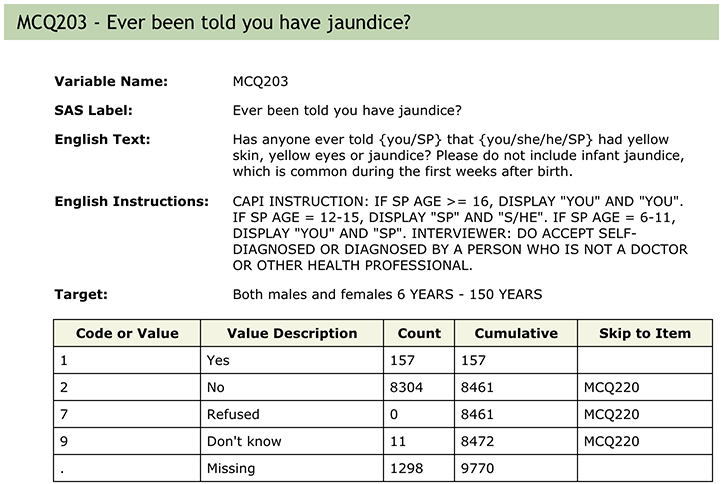
\includegraphics[width=\textwidth,keepaspectratio]{figs/image0copy.png}
\caption{Example from NHANES data dictionary}
\label{fig:image_0}
\end{figure}

\begin{figure}[H]
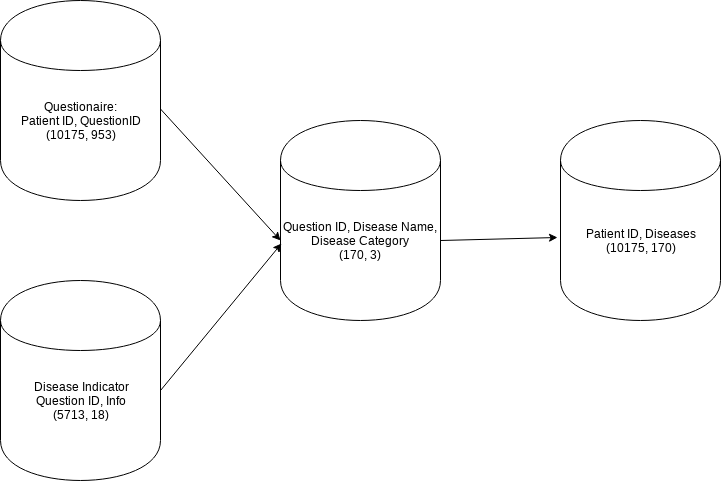
\includegraphics[width=\textwidth,keepaspectratio]{figs/image9.png}
\caption{Data featurization pipeline: patient diseases}
\label{fig:image_9}
\centering
\end{figure}

\begin{figure}[H]
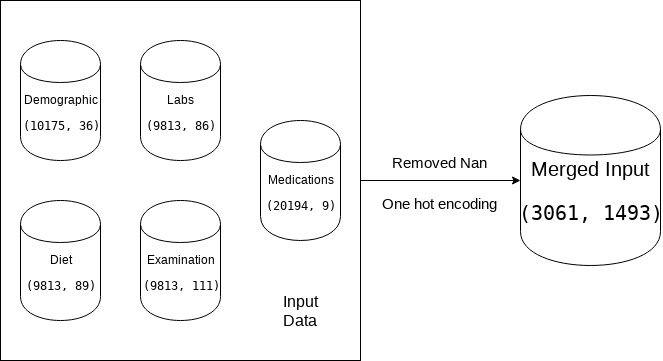
\includegraphics[width=\textwidth,keepaspectratio]{figs/data_preprocessing.png}
\caption{Data featurization pipeline: filtering for patients with complete data}
\label{fig:data_preprocessing}
\centering
\end{figure}

\begin{figure}[H]
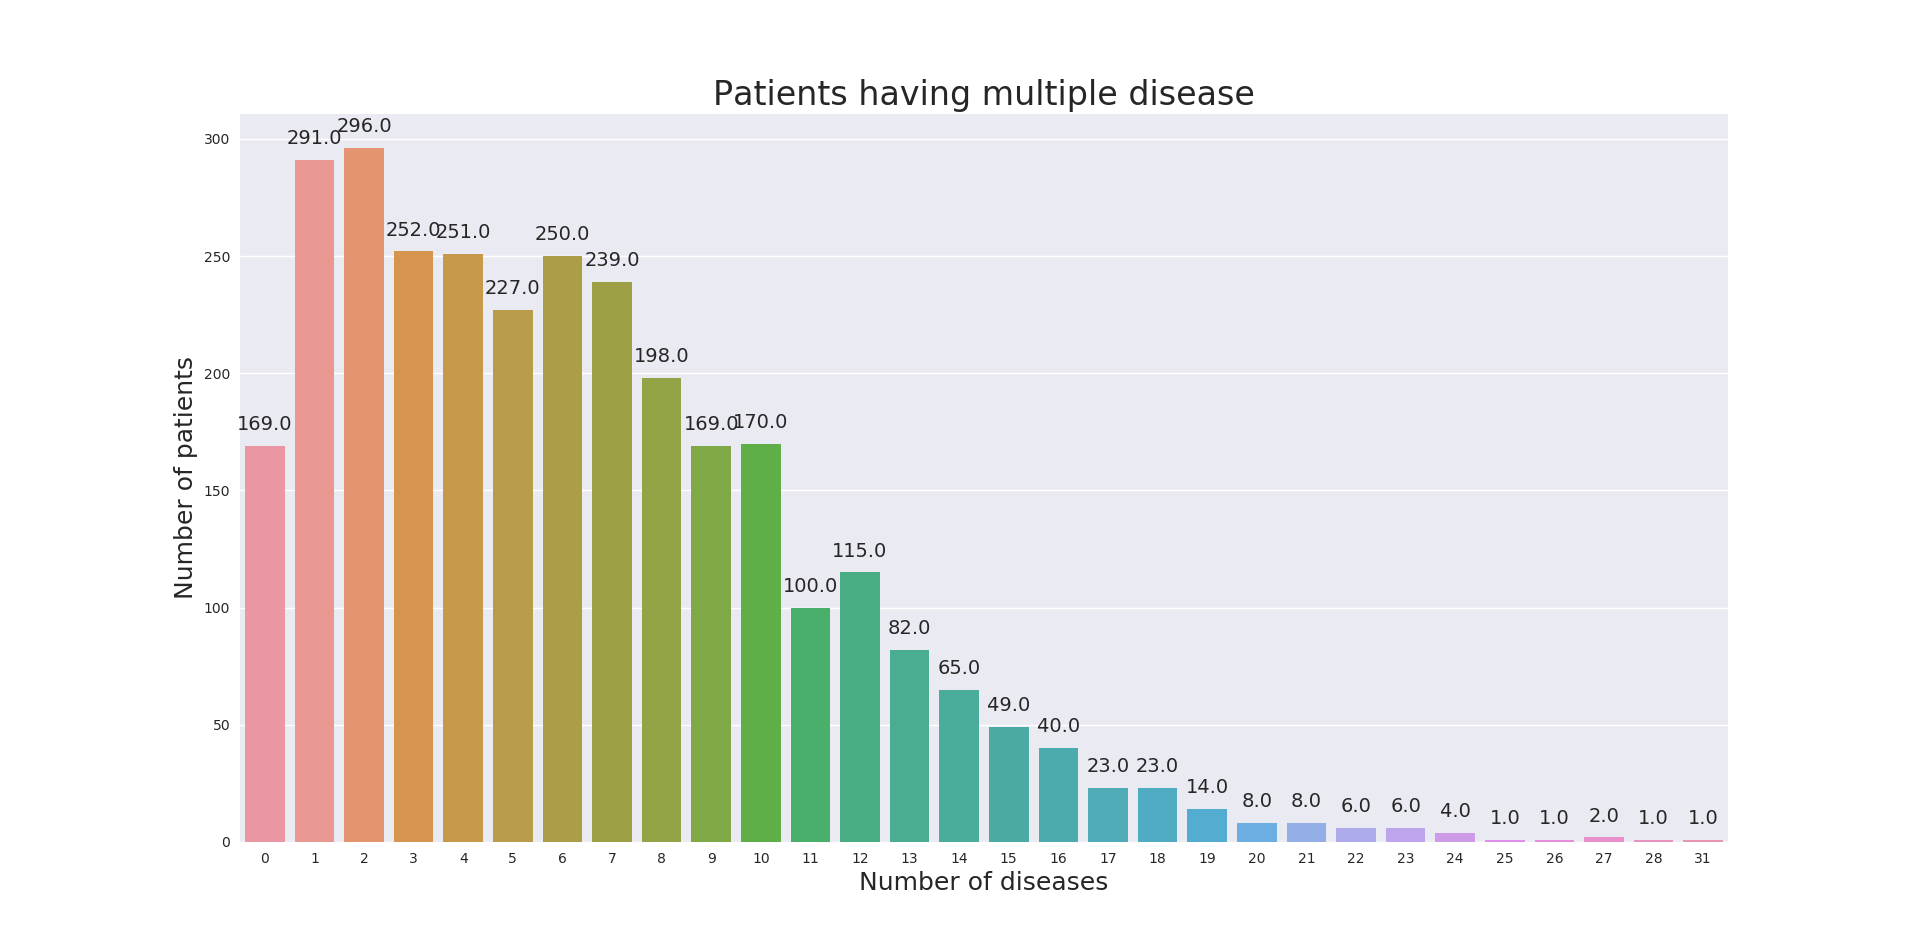
\includegraphics[width=\textwidth,keepaspectratio]{figs/image4.png}
\caption{Most patients had one or more medical condition}
\label{fig:patient_disease_profile}
\centering
\end{figure}

\begin{figure}[H]
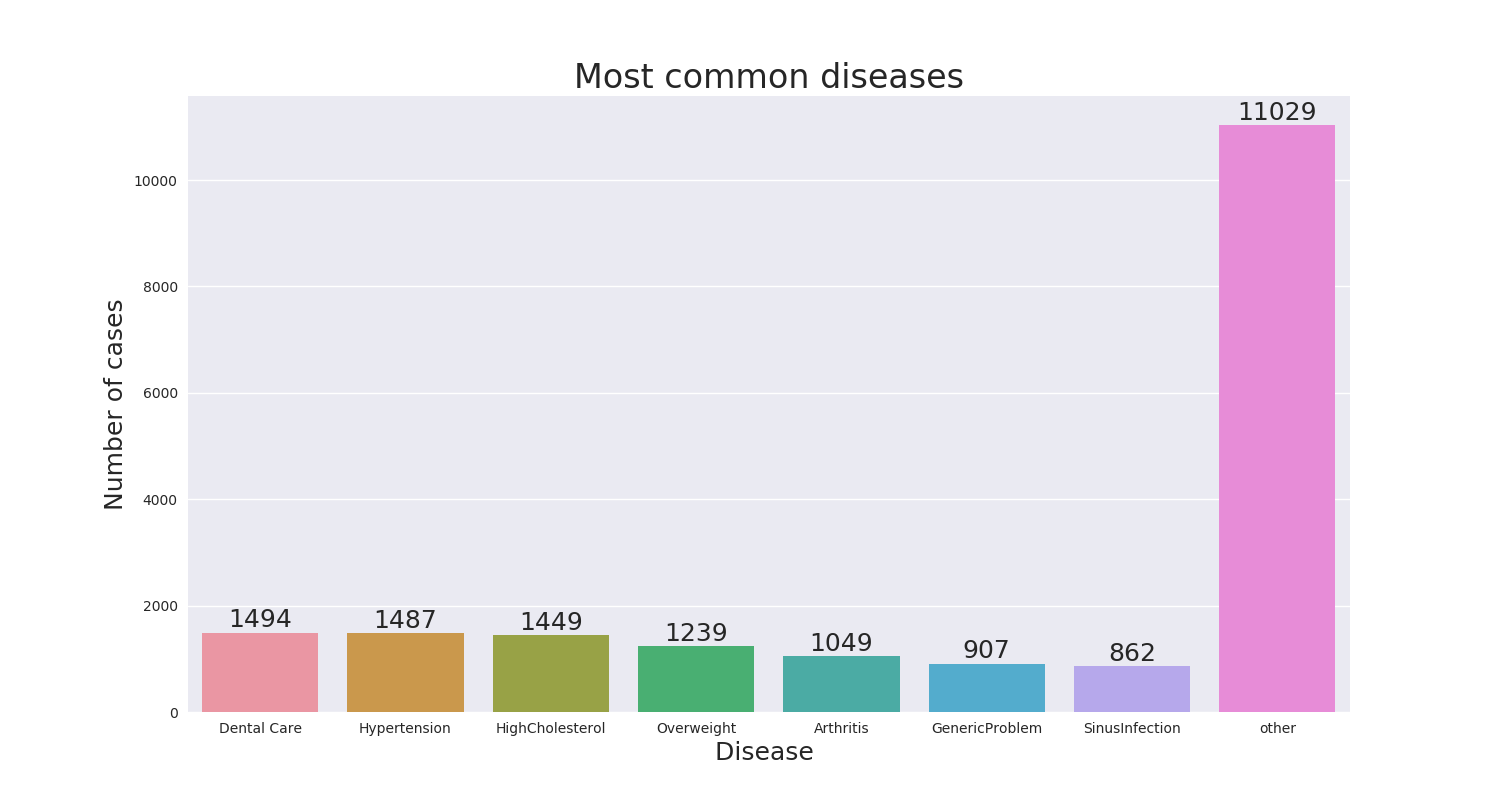
\includegraphics[width=\textwidth,keepaspectratio]{figs/image12.png}
\caption{The most common conditions were chronic ailments}
\label{fig:common_diseases}
\centering
\end{figure}

\begin{figure}[H]
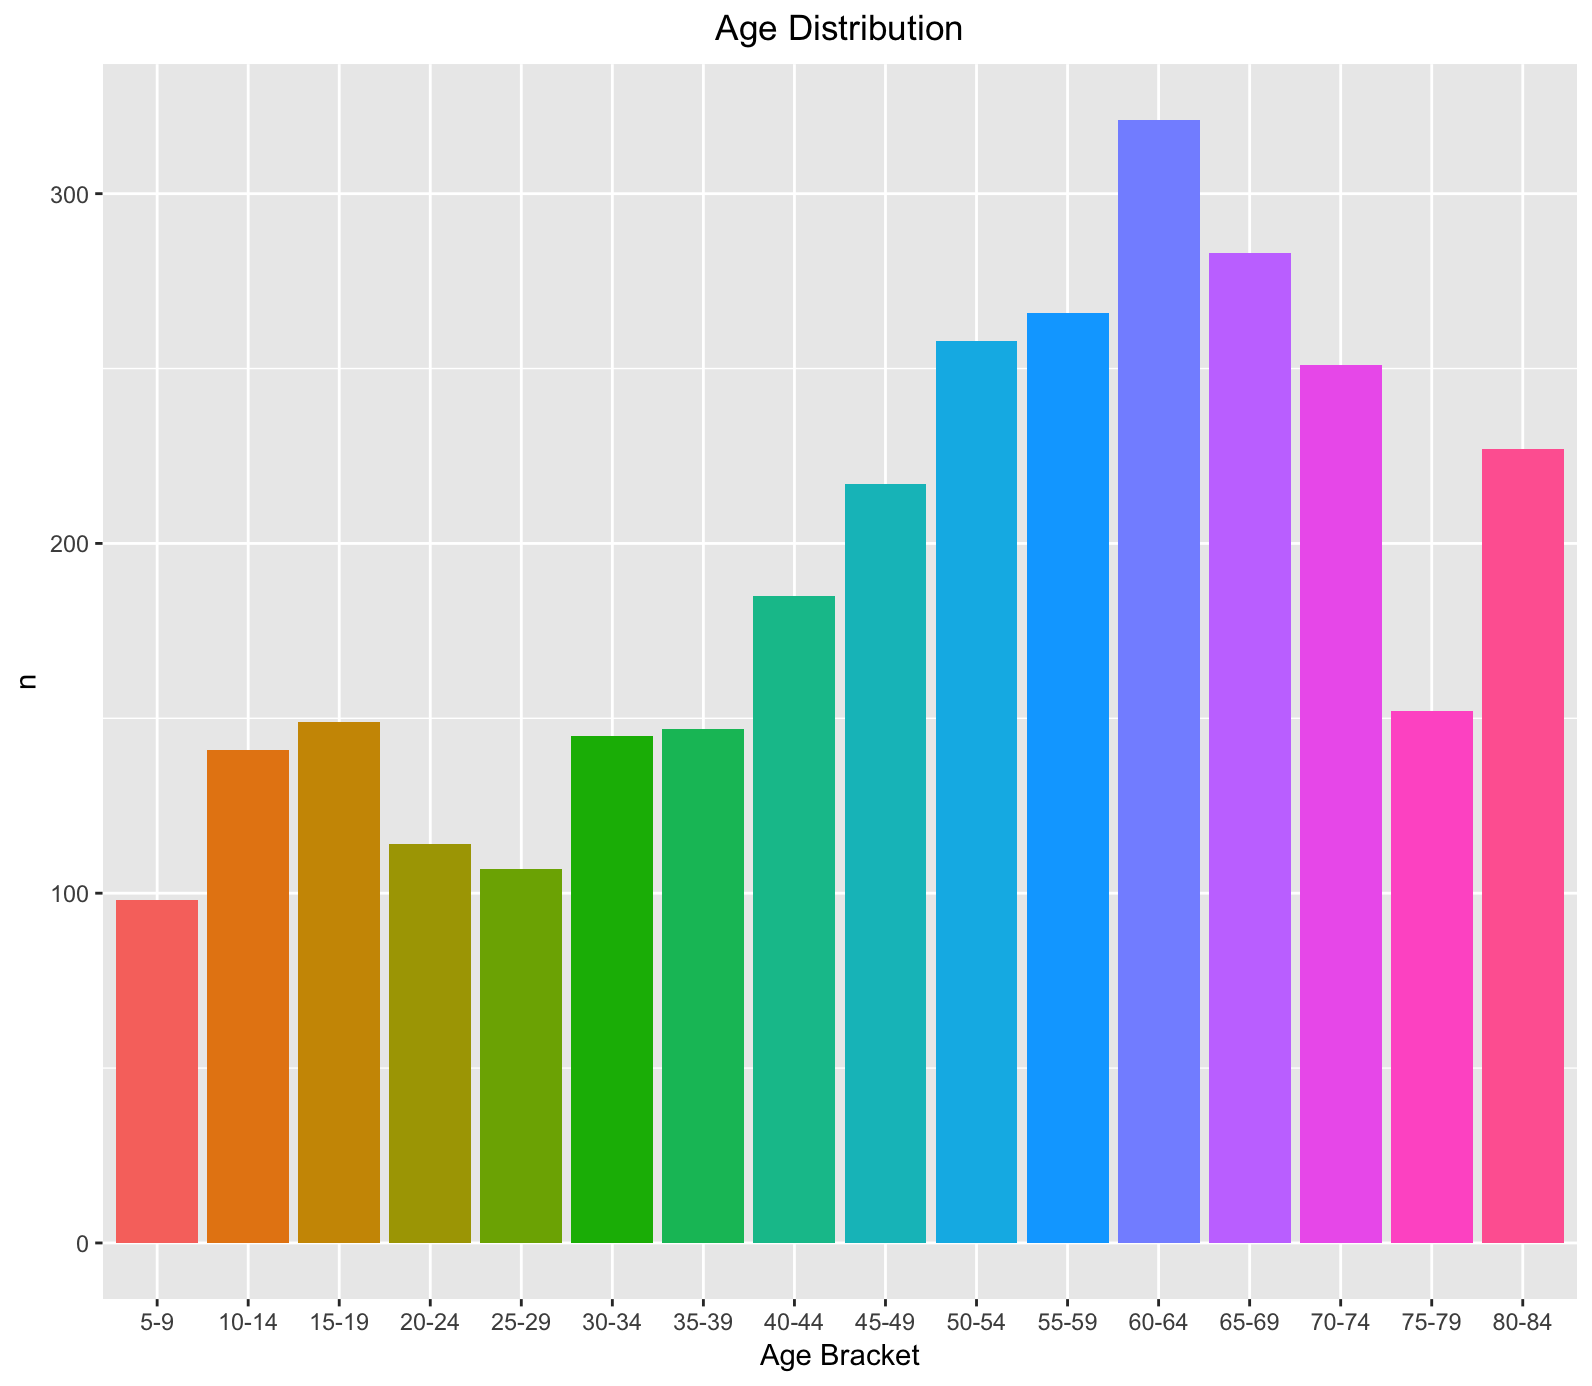
\includegraphics[width=\textwidth,keepaspectratio]{figs/image7.png}
\caption{The most common patient type is female, over the age of 60}
\label{fig:age}
\centering
\end{figure}

\begin{figure}[H]
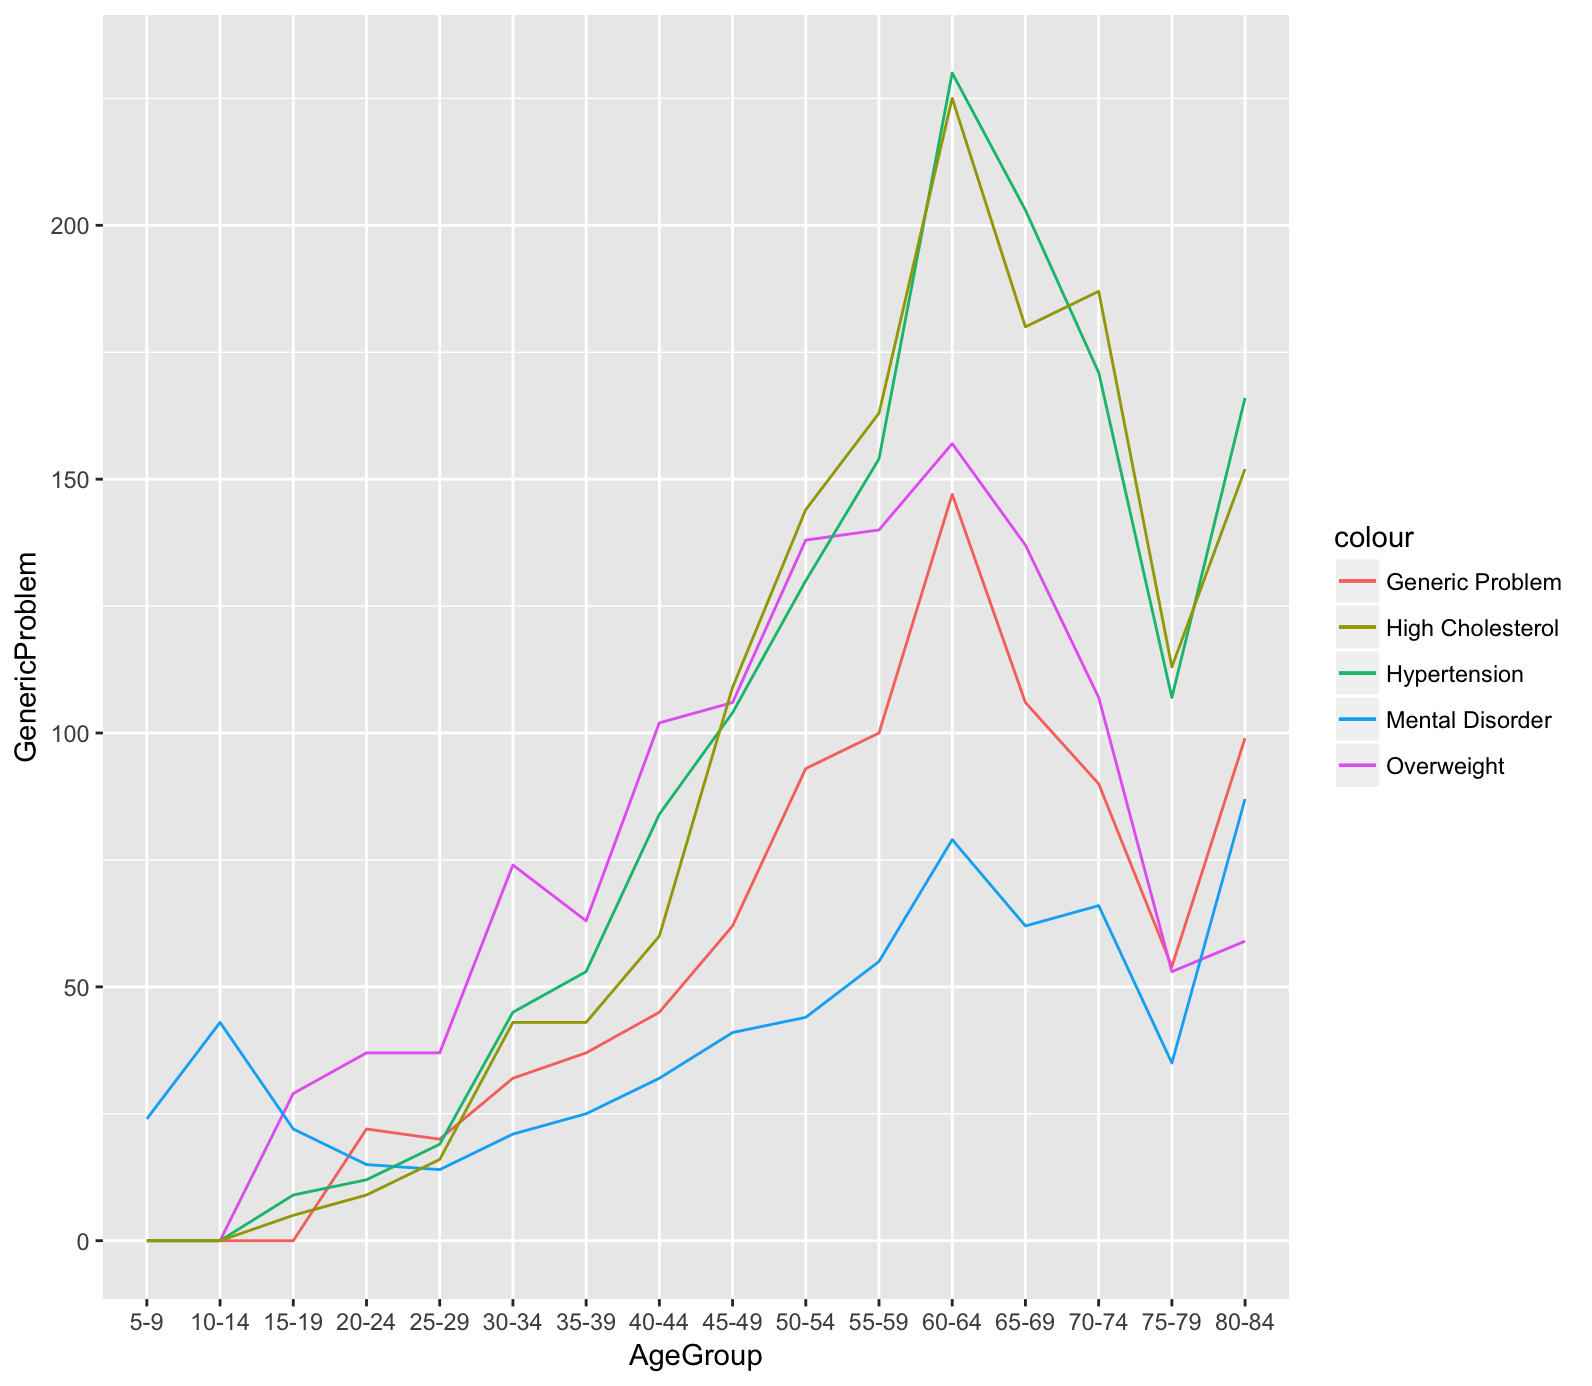
\includegraphics[width=\textwidth,keepaspectratio]{figs/image10.png}
\caption{The frequency of the most common diseases over time}
\label{fig:age_disease}
\centering
\end{figure}


\begin{figure}[H]
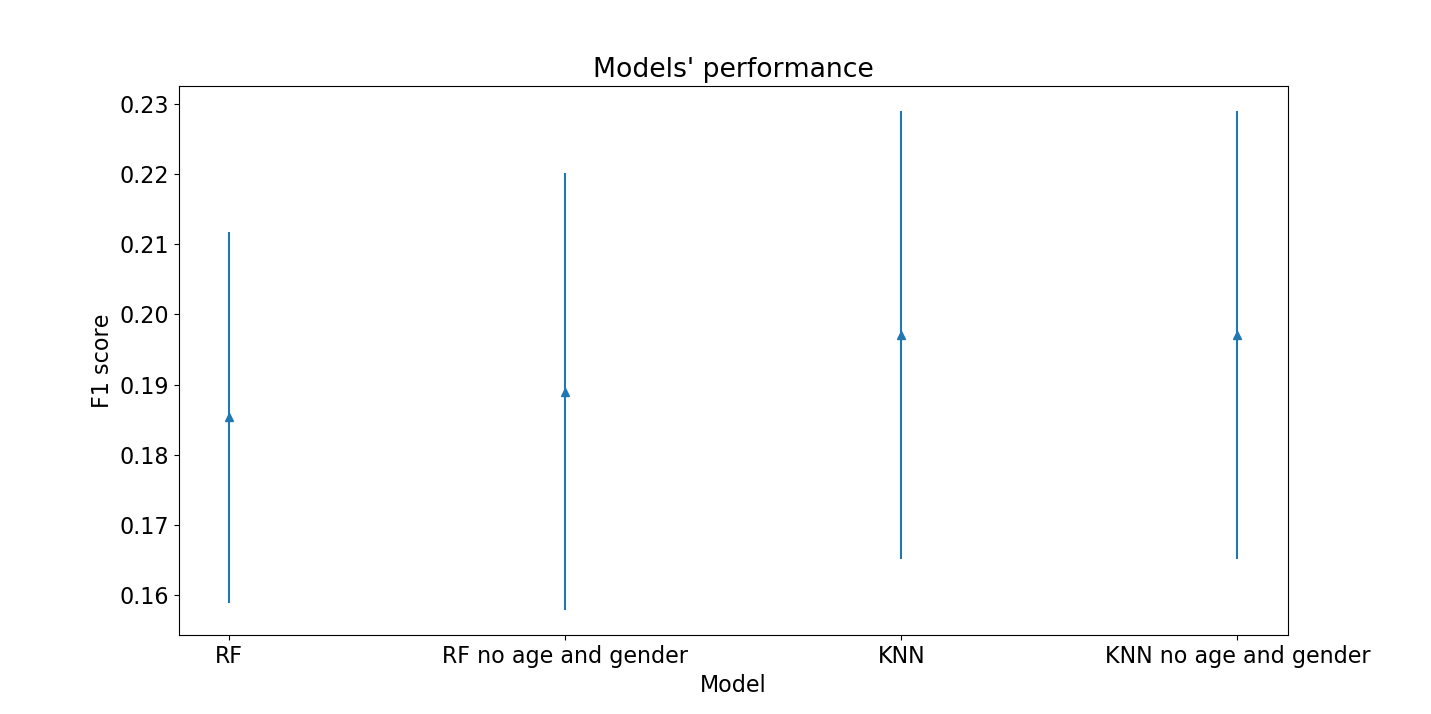
\includegraphics[width=\textwidth,keepaspectratio]{figs/image1.png}
\caption{Initial model performance wasn't very good}
\label{fig:perf1}
\centering
\end{figure}

\begin{figure}[H]
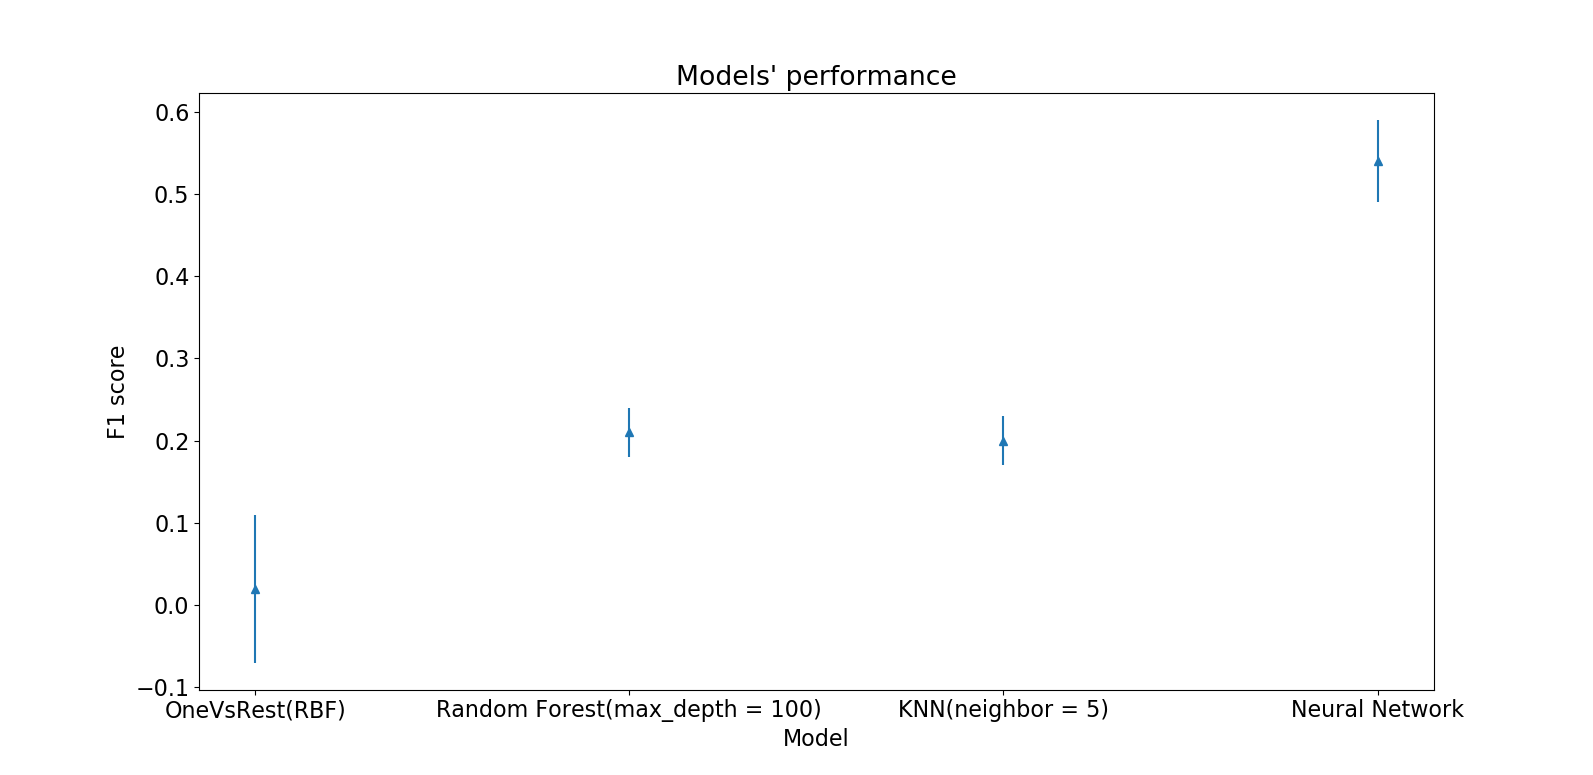
\includegraphics[width=\textwidth,keepaspectratio]{figs/image8.png}
\caption{Neural Network gave the best performance}
\label{fig:perf2}
\centering
\end{figure}

\begin{figure}[H]
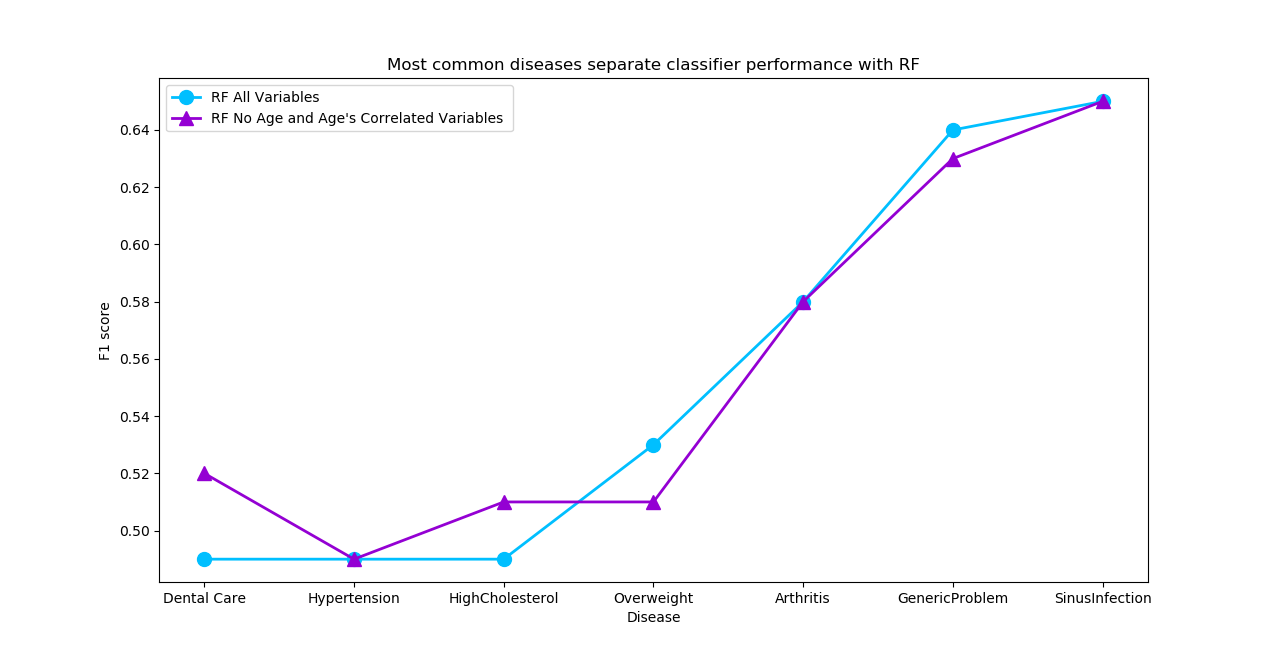
\includegraphics[width=\textwidth,keepaspectratio]{figs/image11.png}
\caption{Fairness Aware Random Forest Performance 1}
\label{fig:fai_rn1}
\centering
\end{figure}

\begin{figure}[H]
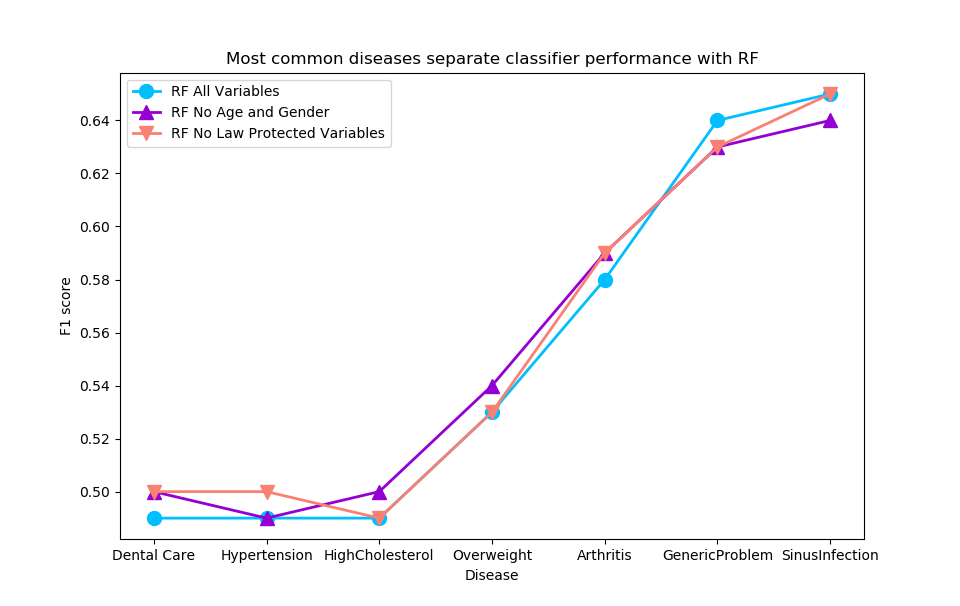
\includegraphics[width=\textwidth,keepaspectratio]{figs/image2.png}
\caption{Fairness Aware Random Forest Performance 2}
\label{fig:fai_rn2}
\centering
\end{figure}

\begin{figure}[H]
\centering
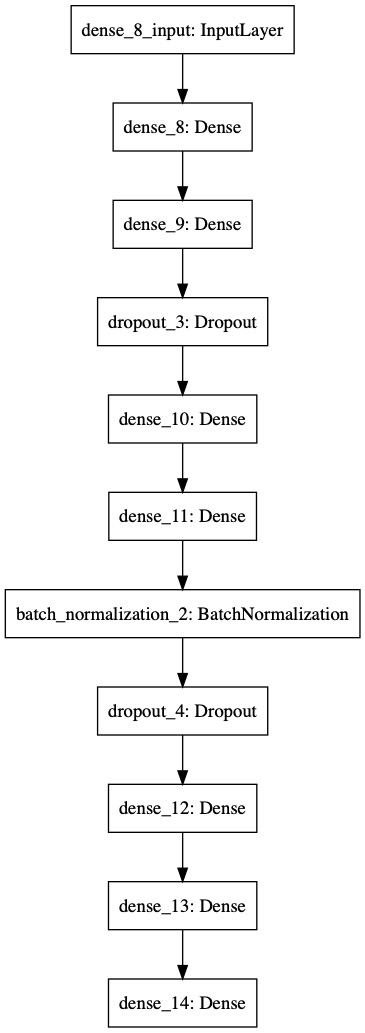
\includegraphics[scale = 0.4,keepaspectratio]{figs/nn.jpg}
\caption{Neural Network Architecture}
\label{fig:nn_arch}
\end{figure}



\end{document}
